%============================================================
\section{Nombre: Energía corrupta.} \label{hab.CorrupEner}
\subsection{Descripción}
El enemigo dispará esferas de tonalli corrupto. las esferas seguirán al jugador durante un periodo de tiempo determinado. Cada esfera reduce la barra de vida del jugador de manera individual al hacer colisión con el jugador. Las esferas se destruyen al hacer contacto con el jugador, al colisionar con cualquier otro objeto o después de un tiempo si no han colisionado con ningún objeto o con el jugador. Las eferas solo afectaran al jugador al hacer contacto con el, si colisionan con otro objeto no afectarán a ese objeto. 
\subsection{Portador}
Tlazoltéotl (ver apartado \ref{per:tlazolteotl}).
\subsection{Esquema}
			Ver figura \ref{fig:energiaC}.
			\begin{figure}
				\centering
				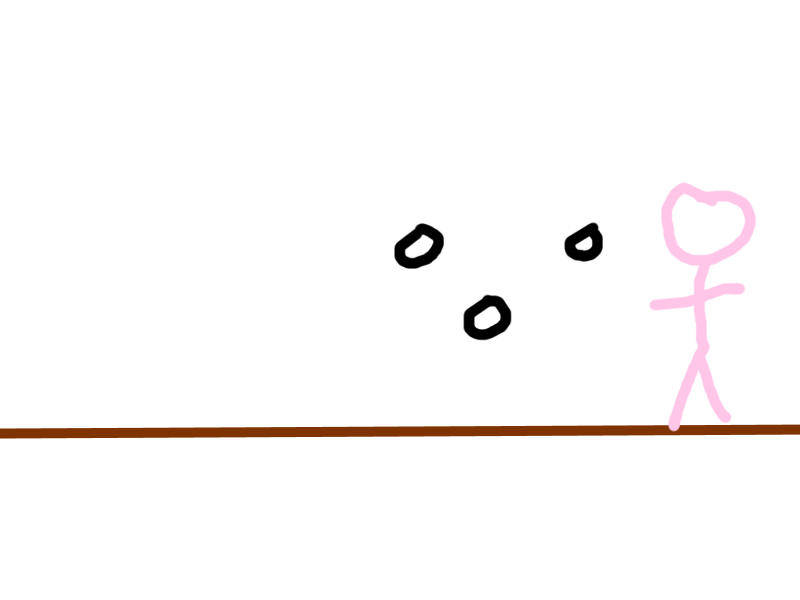
\includegraphics[height=0.2 \textheight]{Imagenes/energiaC}
				\caption{Energía corrupta.}
				\label{fig:energiaC}
			\end{figure}	